\chapter{Background}
\label{ch:background}

The cost of data movement has become the dominant factor of a high performance computing system both in terms of energy consumption and performance. To minimize data movement, applications have to be optimized both for vertical data movement in the memory hierarchy and horizontal data movement between processing units. While microarchitectural technology trends allow the scaling of the number of cores per chip, cache coherence  will likely not scale to the large number of cores due to the traffic overhead of maintaining coherence. In the future, software-managed memory and incoherent caches or scratchpad memory will be prevalent. Thus, application developers need a set of programming abstractions to describe data locality on the new computing ecosystems.

These hardware challenges have been modest enough that the community has largely relied upon compiler technology and software engineering practices to mitigate the coarse-grained effects.  For example, we design applications for MPI to express the coarse-grained data locality where the programmer explicitly represents two levels of computation local (within the node) and message passing (between nodes).  We also deal with cache locality by either relying on the compiler to perform loop blocking on our behalf or manually reorganize loops to explicitly block data for different levels of the cache hierarchy.

The effects were modest enough that these explicit techniques were sufficient to enable codes to perform on different architectures.  However, with the exponential rise in explicit parallelism

\section{Hardware Basis for Locality Optimizations}

\subsection{The End of Classical Performance Scaling}

The year 2004 marked the approximate end of Dennard Scaling. Chip manufacturers could no longer reduce voltages at the historical rates because doing so would have caused the chip to become unreliable. Furthermore, as transistors became smaller, leakage current became a bigger issue. The power dissipated by this leakage current was formerly a small contributor to overall power consumption, but had since become a substantial concern. This meant there was no longer advantage in further reducing operating voltages. Other gains in energy efficiency were still possible; for example, smaller transistors with lower capacitance consume less energy. The inability to reduce the voltages further did mean, however, that clock rates could no longer be increased within the same power budget. Once the practical heat dissipation limit for consumer devices was reached (at approximately 100W of power consumption at the system level) further clock frequency scaling was abandoned.  % This can be seen clearly in the green clock frequency data shown in Figure..... < need to insert>

With the end of voltage scaling, single processing core performance no longer improved with each generation, but performance could be improved, theoretically, by packing more cores into each processor. This multicore approach continues to drive up the theoretical peak performance of the processing chips, and we are on track to have chips with thousands of cores by 2020.  This increase in parallelism via core count is clearly visible in the black trend line in Figure\fix{need figure}.  This is an important development in that programmers outside the small cadre of those with experience in parallel computing must now contend with the challenge of making their codes run effectively in parallel. Parallelism has become everyone?s problem and this will require deep rethinking of the commercial software and algorithm infrastructure. 

Since the loss of Dennard Scaling, a new technology scaling regime has emerged. Due to the laws of electrical resistance and capacitance, a wire?s intrinsic energy efficiency for a fixed-length wire does not improve appreciably as it shrinks down with Moore?s law improvements in lithography as shown in Figure\fix{need fig}. In contrast, the power consumption of transistors continues to decrease as their gate size (and hence capacitance) decreases. Since the energy efficiency of transistors is improving as their sizes shrink, and the energy efficiency of wires is not improving, the point is rapidly approaching where the energy needed to move the data exceeds the energy used in performing the operation on those data.  See Figure\fix{need data locality fig}

\subsection{Data Locality}
Many of the motivations for data locality optimization is rooted in recent hardware architectures trends. 

First among the is the concern that the cost of data movement even within a chip is set to exceed the cost of 

The trend was first observed in the 2008 exascale report, but this has 

Whereas data locality has been a concern for 

Data locality has long been a concern for application development on supercomputers.  Since the advent of caches, vertical data locality has been extraordinarily important for performance.  However, we have largely depended upon automatic management of hardware caches and compiler optimizers to make use of this features.

With the end of Dennard scaling, clock-rates are no longer increasing (figure~\ref{fig:cise-power-clock}) and have been replaced with explicit parallelism.
Figure~\ref{fig:historical} (b) shows a consistent path towards chips with hundreds or even thousands of cores per chip die.  Fortunately, the primary growth in parallelism is on-chip rather than between chips.  Consequently, the available bandwidth between these cores on chip is 10x higher than between nodes, and the latencies are a factor of 10x to 100x lower than between nodes in an HPC system.  The much lower overheads within the chip (compared to off-chip overheads) offer better opportunities to derive performance through increased on-chip parallelism (provided we can express enough parallelism), but the challenge remains daunting.

Parallel computing owes its success to weak scaling between nodes, where the size of the problem solved grows proportionally with the increased parallelism.  The exponential growth in explicit parallelism pushes us towards strong scaling where performance improvements are derived exclusively from applying more parallelism to the same-sized problem.  Certainly, adding cores is fine for increasing compute capacity, but the move towards strong scaling causes communication overheads to become a huge concern.
During the era of exponential scaling of the clock rates within the node took up a lot of the slack when it came to increasing execution rates proportional with the growth of the problem size that supported weak scaling.  For example, in a climate model we could weak scale to increase the problem resolution by a factor of 2x, you must also reduce the time-step size by a factor of 2x to maintain numerical stability of the calculation.  Fortunately, the processor clock rate typically increased by a factor of 2x in that same time interval under old scaling rules.
With the new scaling rules, the 2x improvement in performance must be derived entirely from doubling the performance using increased parallelism.
This is a far more daunting challenge as there are limits to how much parallelism one can express with conventional techniques such as domain decomposition before the communication overheads kill performance.

The research community is starting to look at more aggressive techniques that depart from our traditional bulk-synchronous or SPMD (Single Program Multiple Data) model for parallelism.   One common approach involves "functional partitioning" where different solvers of the simulation are executed concurrently to overcome these granularity and processor speed limitations.   For example a combustion code or climate simulation would concurrently schedule parts of the memory bandwidth intensive fluid dynamics compilation concurrently with the FLOP-intensive chemistry calculations -- thereby increasing the number of utilized processors and hence overall throughput without relying on increased domain decomposition.  In addition, you can use very low-overhead inter-core message queues to reduce communication overhead within a chip as we did for the Green Flash chip-multiprocessor design~\cite{GreenFlash}.  However, conventional C and Fortran language semantics make it difficult to manage this kind of parallelism, so there is a new thrust to explore language semantics that support asymmetric and asynchronous approaches to achieving strong-scaling performance improvements from explicit parallelism.  Successful demonstration of such parallelization procedures for a range of leading extreme-scale applications can then be utilized by other similar codes at smaller scales, which will accelerate development efforts for the entire field.

\begin{figure}\begin{centering}
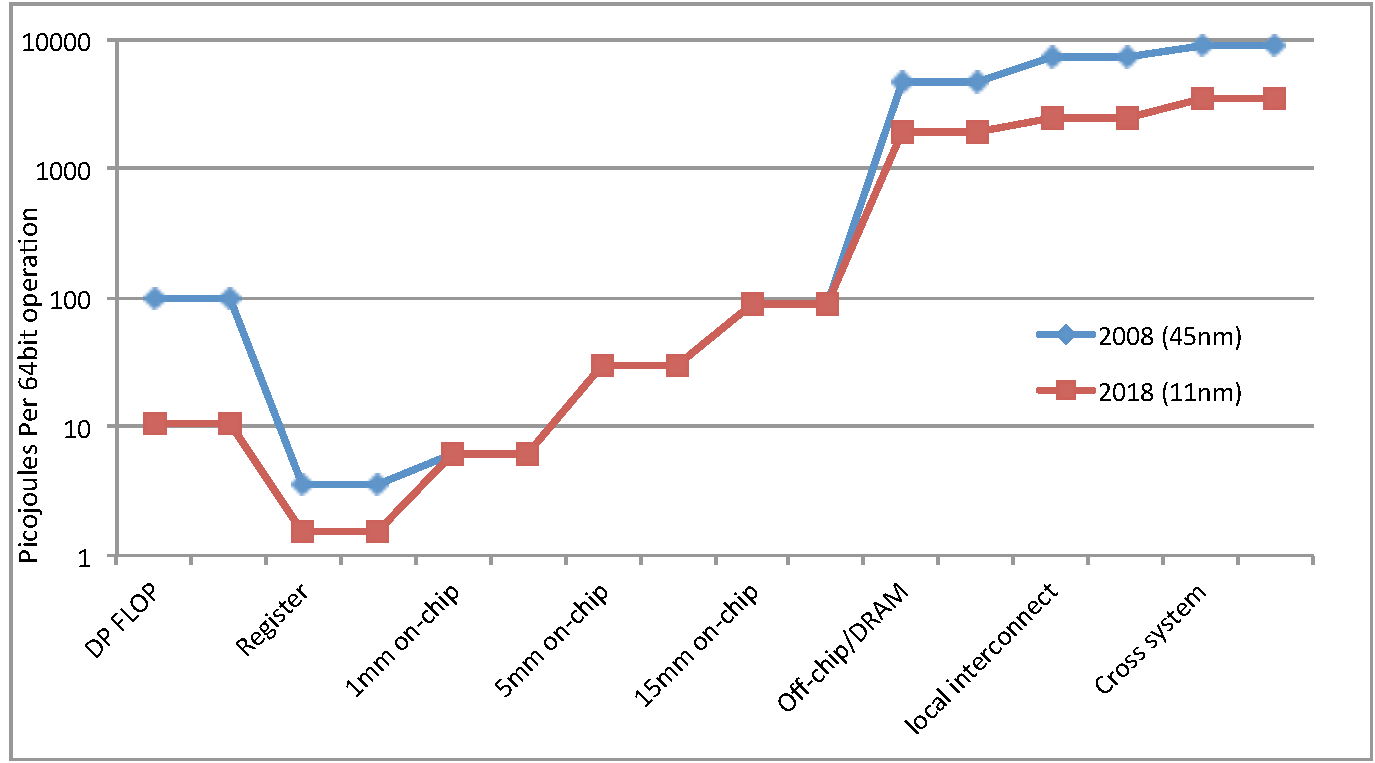
\includegraphics[width=0.95\columnwidth]{background/figures/DataMovement2.pdf}
\caption{Data movement is overtaking computation as the most dominant cost of a system both in terms of dollars and in terms of energy consumption.  Consequently, we should be more explicit about reasoning about data movement. This diagram shows the cost of operations or data movement for a 64-bit operand.  By 2018, the cost of moving a 64-bit operand a mere 5mm across the chip will exceed that of a floating point operation that uses that operand. {\em The FPU and Register File energy model is computed from Tensilica's RTL design for an LX4 core with FPU.  The data movement on-chip is based on a standard resistive/capacitive model with simple signal regeneration.  The DRAM is based on Micron's projections for DDR parts.  The interconnect model is based on extrapolating historical improvements in optical transceiver efficiency and data rates.}}
\label{fig:datamovement}
\end{centering}\end{figure}

\subsection{Performance Heterogeneity}

We have evolved a parallel computing infrastructure that is optimized for bulk-synchronous execution models.  It implicitly assumes that every processing element is identical and operates at the same performance.  However, performance projections out to exascale in figure~\ref{fig:energy-per-flop} show that the only technological path that has a hope of achieving exascale by 2020 involves a heterogeneous architecture consisting of both lightweight and heavyweight cores.  Even if you are not enthusiastic about the complexity of programming heterogeneous compute engines (hybrid/accelerated computing), application developers will still need to confront heterogeneity even for homogenous processor technology.
Emerging adaptive algorithms, near-threshold voltage operation, and clock-speed throttling challenge current assumptions of uniformity.
Since the most energy-efficient FLOP is the one you do not perform, there is increased interest in using adaptive and irregular algorithms to apply computation only where it is required, and also to reduce memory requirements.  Even for systems with homogeneous computation on homogeneous cores, new fine-grained power management makes homogeneous cores look heterogeneous.  For example thermal throttling on Intel Sandybridge enables the core to opportunistically sprint to a higher clock frequency until it gets too hot, but the implementation cannot guarantee deterministic clock rate because chips heat up at different rates.  In the future, nonuniformities in process technology and Near-Threshold-Voltage (NTV) for ultra-low-power logic will create non-uniform operating characteristics for cores on a chip multiprocessor.  Fault resilience will also introduce inhomogeneity in execution rates as even hardware error correction is not instantaneous, and software-based resilience will introduce even larger performance heterogeneity.

So even homogeneous hardware will look increasingly heterogeneous in future technology generations.  Consequently, we can no longer depend on homogeneity, which presents an existential challenge to bulk-synchronous execution models.  This has renewed interest in alternative execution models that are better able to accommodate performance non-uniformity.  For example ETI Swarm, ParalleX, and Charm++ posit a completely asynchronous execution methodology that enables parallelism to be derived from concurrent scheduling of independent work rather than just by data decomposition.  These techniques that borrow much from coarse-grained dataflow methods are garnering renewed interest because of their ability to flexibly schedule work and to accommodate state migration to correct load imbalances and failures for this kind of functional partitioning model.



Performance heterogeneity offers a number of challenges to conventional approaches to data management.

1) Breaking lexical order execution of programs
2) Balancing data locality with optimal scheduling
3) Isolation of side-effects
4) Abstractions for over-decomposition

